\chapter*{Proposition 29}


\begin{figure*}[ht]
    \begin{center}
    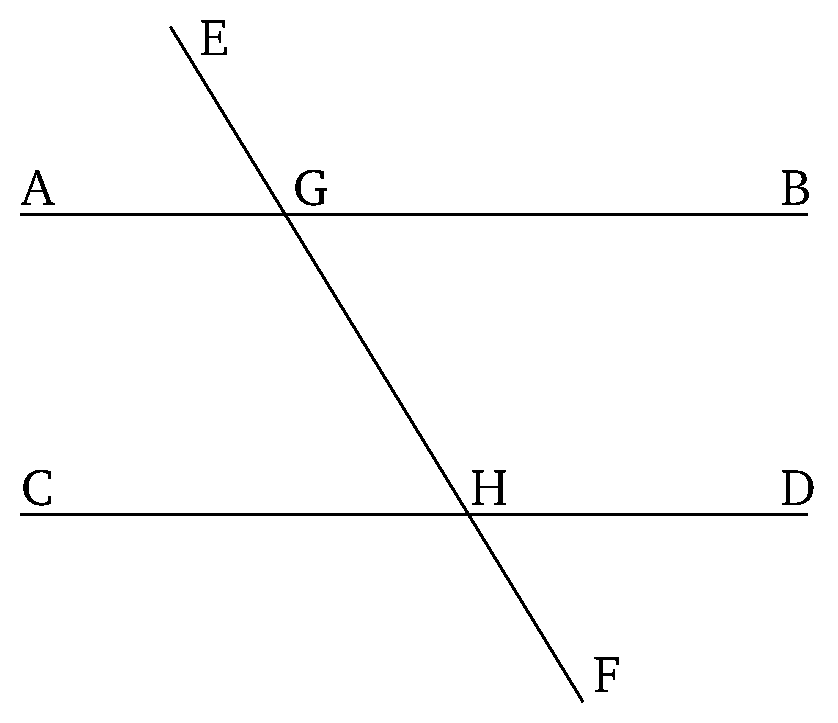
\includegraphics[width=0.5\linewidth]{figures/fig28e.eps}
    \label{fig:prop_29}
    \end{center}
\end{figure*}

A straight-line falling across  parallel straight-lines makes the alternate angles
equal to one another,  the external (angle) equal to the internal and
opposite (angle), and the (sum of the) internal (angles) on the same side equal to
two right-angles.

For let the straight-line $EF$ fall across the parallel straight-lines $AB$ and $CD$.
I say that it makes the  alternate angles, $AGH$ and $GHD$,  equal,  the
external angle $EGB$ equal to the internal and opposite (angle) $GHD$,
and the (sum of the) internal (angles) on the same side, $BGH$ and $GHD$, equal to
two right-angles.

For if $AGH$ is unequal to $GHD$ then one of them is greater. Let $AGH$ be greater.
Let $BGH$ have been added to both. Thus, (the sum of) $AGH$ and $BGH$ is greater
than (the sum of) $BGH$ and $GHD$. But, (the sum of) $AGH$ and $BGH$ is equal to two right-angles
[Prop~1.13]. Thus,  (the sum of) $BGH$ and $GHD$ is [also] less than two right-angles. 
But (straight-lines) being produced to infinity from (internal angles whose sum is) less than
two right-angles meet together [Post.~\ref{post:5}]. Thus, $AB$ and $CD$, being produced to
infinity, will meet together. But they do not meet, on account of
them (initially) being assumed parallel (to one another) [Def.~\ref{def:23}]. Thus, $AGH$ is not unequal to $GHD$. Thus, (it is) equal. But, $AGH$ is equal to $EGB$ [Prop.~1.15]. 
And $EGB$ is thus also equal to $GHD$.
Let $BGH$
be added to both. Thus, (the sum of) $EGB$ and $BGH$ is equal to (the sum of) $BGH$ and $GHD$.
But, (the sum of) $EGB$ and $BGH$ is equal to two right-angles [Prop.~1.13]. 
Thus, (the sum of) $BGH$ and $GHD$ is also equal to two right-angles.

Thus, a straight-line falling across parallel straight-lines makes the alternate angles
equal to one another,  the external (angle) equal to the internal and
opposite (angle), and the (sum of the) internal (angles) on the same side equal to
two right-angles. (Which is) the very thing it was required to show.


\section*{Commentary}

\begin{proposition}\label{proposition_29}\lean{Elements.Book1.proposition_29}\leanok
    If
\end{proposition}
\begin{proof}
    \uses{proposition_13,proposition_15}\leanok
\end{proof}
